%\section{Simulation Study}

\subsection{Simulation Procedure}

To test the performance of Algorithm \ref{alg:EM-VRSO}, we ran eight simulation experiments. For a given experiment, we simulated $T \in \{10^3,10^5\}$ observations from an HMM with $N \in \{3,6\}$ hidden states and observations $y_t \in \bbR^d$, with $d \in \{3,6\}$. All possible combinations of $T$, $N$, and $d$ comprised a total of $2^3 = 8$ experiments. For each experiment, we simulated five data sets. For every experiment and data set, $Y_t \mid X_t = i$ followed a normal distribution with mean $\mu^{(i)}$ and covariance matrix $\bfSigma^{(i)}$. We defined $\mu^{(i)}$ and $\bfSigma^{(i)}$ for every data set as $\mu^{(i)} \sim \calN(0,I)$ and $\bfSigma^{(i)} = \text{diag}[\exp(-2)]$ for $i \in \{1,\ldots,N\}$ where $I$ is the identity matrix. This simulation procedure resulted in relatively well separated state-dependent distributions. For example, when $N = 3$, the Euclidean distance between any pair of means within any of the five data sets ranged between 1.0 and 4.0 for $d = 3$ and between 2.0 and 4.7 for $d = 6$.
%
We set the transition probability matrices of the generating process to depend upon $T$ so that the expected number of total transitions was 100 for all experiments. Our purpose in keeping the expected number of transitions fixed was to induce a high degree of sequential dependence while simultaneously encouraging each hidden state to be visited in the simulated time series. This decision also simulates sequences of observations that are sampled at either low ($T=10^3$) or high ($T=10^5$) frequencies.
%
Denote the true transition probability matrix from an experiment with $T$ observations and $N$ hidden states as $\bfGamma_{T,N}$. We defined $\bfGamma_{10^3,3} \in \bbR^{3 \times 3}$ to have diagonal elements of 0.9 and off-diagonal elements of 0.05, $\bfGamma_{10^3,6} \in \bbR^{6 \times 6}$ to have diagonal elements of 0.9 and off-diagonal elements of 0.02, $\bfGamma_{10^5,3} \in \bbR^{3 \times 3}$ to have diagonal elements of 0.999 and off-diagonal elements of $5 \times 10^{-4}$, and $\bfGamma_{10^3,6} \in \bbR^{6 \times 6}$ to have diagonal elements of 0.999 and off-diagonal elements of $2 \times 10^{-4}$. 
%
\iffalse
\begin{gather*}
    \bfGamma_{10^3,3} = 
    \begin{pmatrix} 
        0.9 & 0.05 & 0.05 \\
        0.05 & 0.9 & 0.05 \\
        0.05 & 0.05 & 0.9
    \end{pmatrix},
    \qquad
    \bfGamma_{10^3,6} = 
    \begin{pmatrix} 
        0.9  & 0.02 & 0.02 & 0.02 & 0.02 & 0.02 \\
        0.02 & 0.9  & 0.02 & 0.02 & 0.02 & 0.02 \\
        0.02 & 0.02 & 0.9  & 0.02 & 0.02 & 0.02 \\
        0.02 & 0.02 & 0.02 & 0.9  & 0.02 & 0.02 \\
        0.02 & 0.02 & 0.02 & 0.02 & 0.9  & 0.02 \\
        0.02 & 0.02 & 0.02 & 0.02 & 0.02 & 0.9  \\
    \end{pmatrix},
    \\
    \bfGamma_{10^5,3} = 
    \begin{pmatrix} 
        0.999 & 0.0005 & 0.0005 \\
        0.0005 & 0.999 & 0.0005 \\
        0.0005 & 0.0005 & 0.999
    \end{pmatrix}
    \qquad
    \bfGamma_{10^5,6} = 
    \begin{pmatrix} 
        0.999  & 0.0002 & 0.0002 & 0.0002 & 0.0002 & 0.0002 \\
        0.0002 & 0.999  & 0.0002 & 0.0002 & 0.0002 & 0.0002 \\
        0.0002 & 0.0002 & 0.999  & 0.0002 & 0.0002 & 0.0002 \\
        0.0002 & 0.0002 & 0.0002 & 0.999  & 0.0002 & 0.0002 \\
        0.0002 & 0.0002 & 0.0002 & 0.0002 & 0.999  & 0.0002 \\
        0.0002 & 0.0002 & 0.0002 & 0.0002 & 0.0002 & 0.999  \\
    \end{pmatrix}.
\end{gather*}
\fi
%
We randomly defined the initial distribution as $\bfdelta \sim \text{dir}(\onevec_N)$ for every experiment and data set.

\subsection{Optimization Procedure}

We estimated the parameters of the generating model for all five data sets and all eight experiments using six different versions of Algorithm \ref{alg:EM-VRSO}. In particular, we used $A \in \{\text{SVRG, SAGA}\}$, and for each value of $A$, we used the combinations $\{P = \texttt{False}, ~ M = T\}$, $\{P = \texttt{True}, ~ M = T\}$, and $\{P = \texttt{True}, ~ M = 10T\}$. Recall that setting $P = \texttt{True}$ corresponds to integrating a partial E step into the variance-reduced stochastic M step. The variable $M$ corresponds to the number of iterations of SAGA or SVRG that are performed at each M step of the algorithm. It is natural to set $M=T$ to approximately balance the computational load of the E step and the M step. Nonetheless, we ran an experiment with $M=10T$ and $P = \texttt{True}$ to test the algorithm when the majority of the computational load was placed on the combined partial E / stochastic M step. As a baseline, we also estimated the HMM parameters using direct likelihood maximization via three gradient-based methods: BFGS \citep{Fletcher:2000}, the conjugate gradient method \citep{Fletcher:1964}, and full-batch gradient descent. The model used in our simulation study has closed-form solutions to the M step of the Baum-Welch algorithm. However, we did not include the standard Baum-Welch algorithm as a baseline method because we did not want to rely on closed-form solutions to the M step. If such solutions exist in practice, we recommend using either the standard Baum-Welch algorithm or the Baum-Welch algorithm with a partial E step \citep{Neal:1998}.

We sampled a total of five random parameter initializations for each data set / experiment pair, and then ran all nine optimization algorithms on every parameter initialization. Each parameter initialization was re-used for each algorithm to ensure consistency. Throughout the optimization procedure, we assumed that $\bfSigma^{(i)}$ was diagonal for all $i \in \{1,\ldots,N\}$, which is in line with the generating model described above. Further, we reparameterized $\bfSigma^{(i)}$ as 
%
$\bfSigma^{(i)} = \text{diag}\left[\exp(\boldsymbol{\rho}^{(i)})\right]$
%
and performed inference on $\boldsymbol{\rho}^{(i)} = \begin{pmatrix} \rho^{(i)}_1 & \ldots & \rho^{(i)}_d \end{pmatrix}$ for $i = 1,\ldots,N$, which is unconstrained. 
%
Let $\bar y$ denote the sample mean and $\bfQ$ denote the sample covariance of the observation sequence $\{y_t\}_{t=1}^T$. We initialized $\bftheta_0 = \{\mu^{(i)}_0,\boldsymbol{\rho}^{(i)}_0\}_{i=1}^N$ as
%
$\mu^{(i)}_0 \sim \calN(\bar y, \text{diag}(\bfQ))$ and $\boldsymbol{\rho}^{(i)}_0 \sim \calN\left(\log(\text{diag}(\bfQ)), 2I \right)$ for $i = 1,\ldots,N$.
%
We initialized $\bfnu_0$ as
%
$\nu^{(i)}_0 \sim \calN(0,1)$ for $i = 2,\ldots,N$ and we initialized $\bfeta_0$ as
%
$\eta^{(i,j)}_0 \sim \calN(-2,2^2)$ for $i,j = 1,\ldots,N$, where $i \neq j$.
%
All six algorithms were initialized with step sizes of $\lambda_{\bftheta} = 1/3 \hat L_G$ and $\lambda_{\bfeta,\bfnu} = 1/3 \hat L_H$. The Lipschitz constants were initialized as $\hat L_G = \hat L_H = 100/3$ and updated during the optimization routine according to the procedure from section \ref{subsec:est_L}. 
%
All algorithms and baselines were run for a total of 12 hours on the Compute Canada Cedar cluster on nodes with 16GB of RAM.
%
All baselines were implemented using the Scipy library in Python \citep{Virtanen:2019}, and we implemented Algorithm \ref{alg:EM-VRSO} using a custom Python script.

We employed several measures to fairly compare the performance of each optimization algorithm. To account for differences in speed due to implementation discrepancies, we measured computational complexity in epochs in addition to raw computation time. We define one epoch as either $T$ evaluations of Equations (\ref{eqn:tilde_alpha} -- \ref{eqn:tilde_xi}) in the E step of Algorithm \ref{alg:EM-VRSO}, $T$ stochastic gradient evaluations in the M step of Algorithm \ref{alg:EM-VRSO}, or one gradient evaluation in the full-gradient baseline algorithms. We estimated the true maximum likelihood parameters $\bfphi^*$ for each data set / experiment pair using the parameters from the best-performing optimization algorithm and initialization after 12 hours. Convergence was defined as the point when the gradient norm of the log-likelihood (divided by $T$) was less than $10^{-2}$. The tolerance was set to $10^{-2}$ because it was the lowest tolerance that all algorithms regularly converged to within 12 hours. Even though each algorithm was run for a full 12 hours, we denoted the epoch and time when each algorithm either converged or finished running as the moment of ``termination".

\subsection{Simulation Results}

The results from the simulation study are shown in Figures 2--4. We were primarily focused on the big-data setting and thus only present results from experiments with $T=10^5$ in the main text. All figures associated with experiments for $T=10^3$ can be found in Supplement A.

\begin{figure}%[ht]
    \centering
    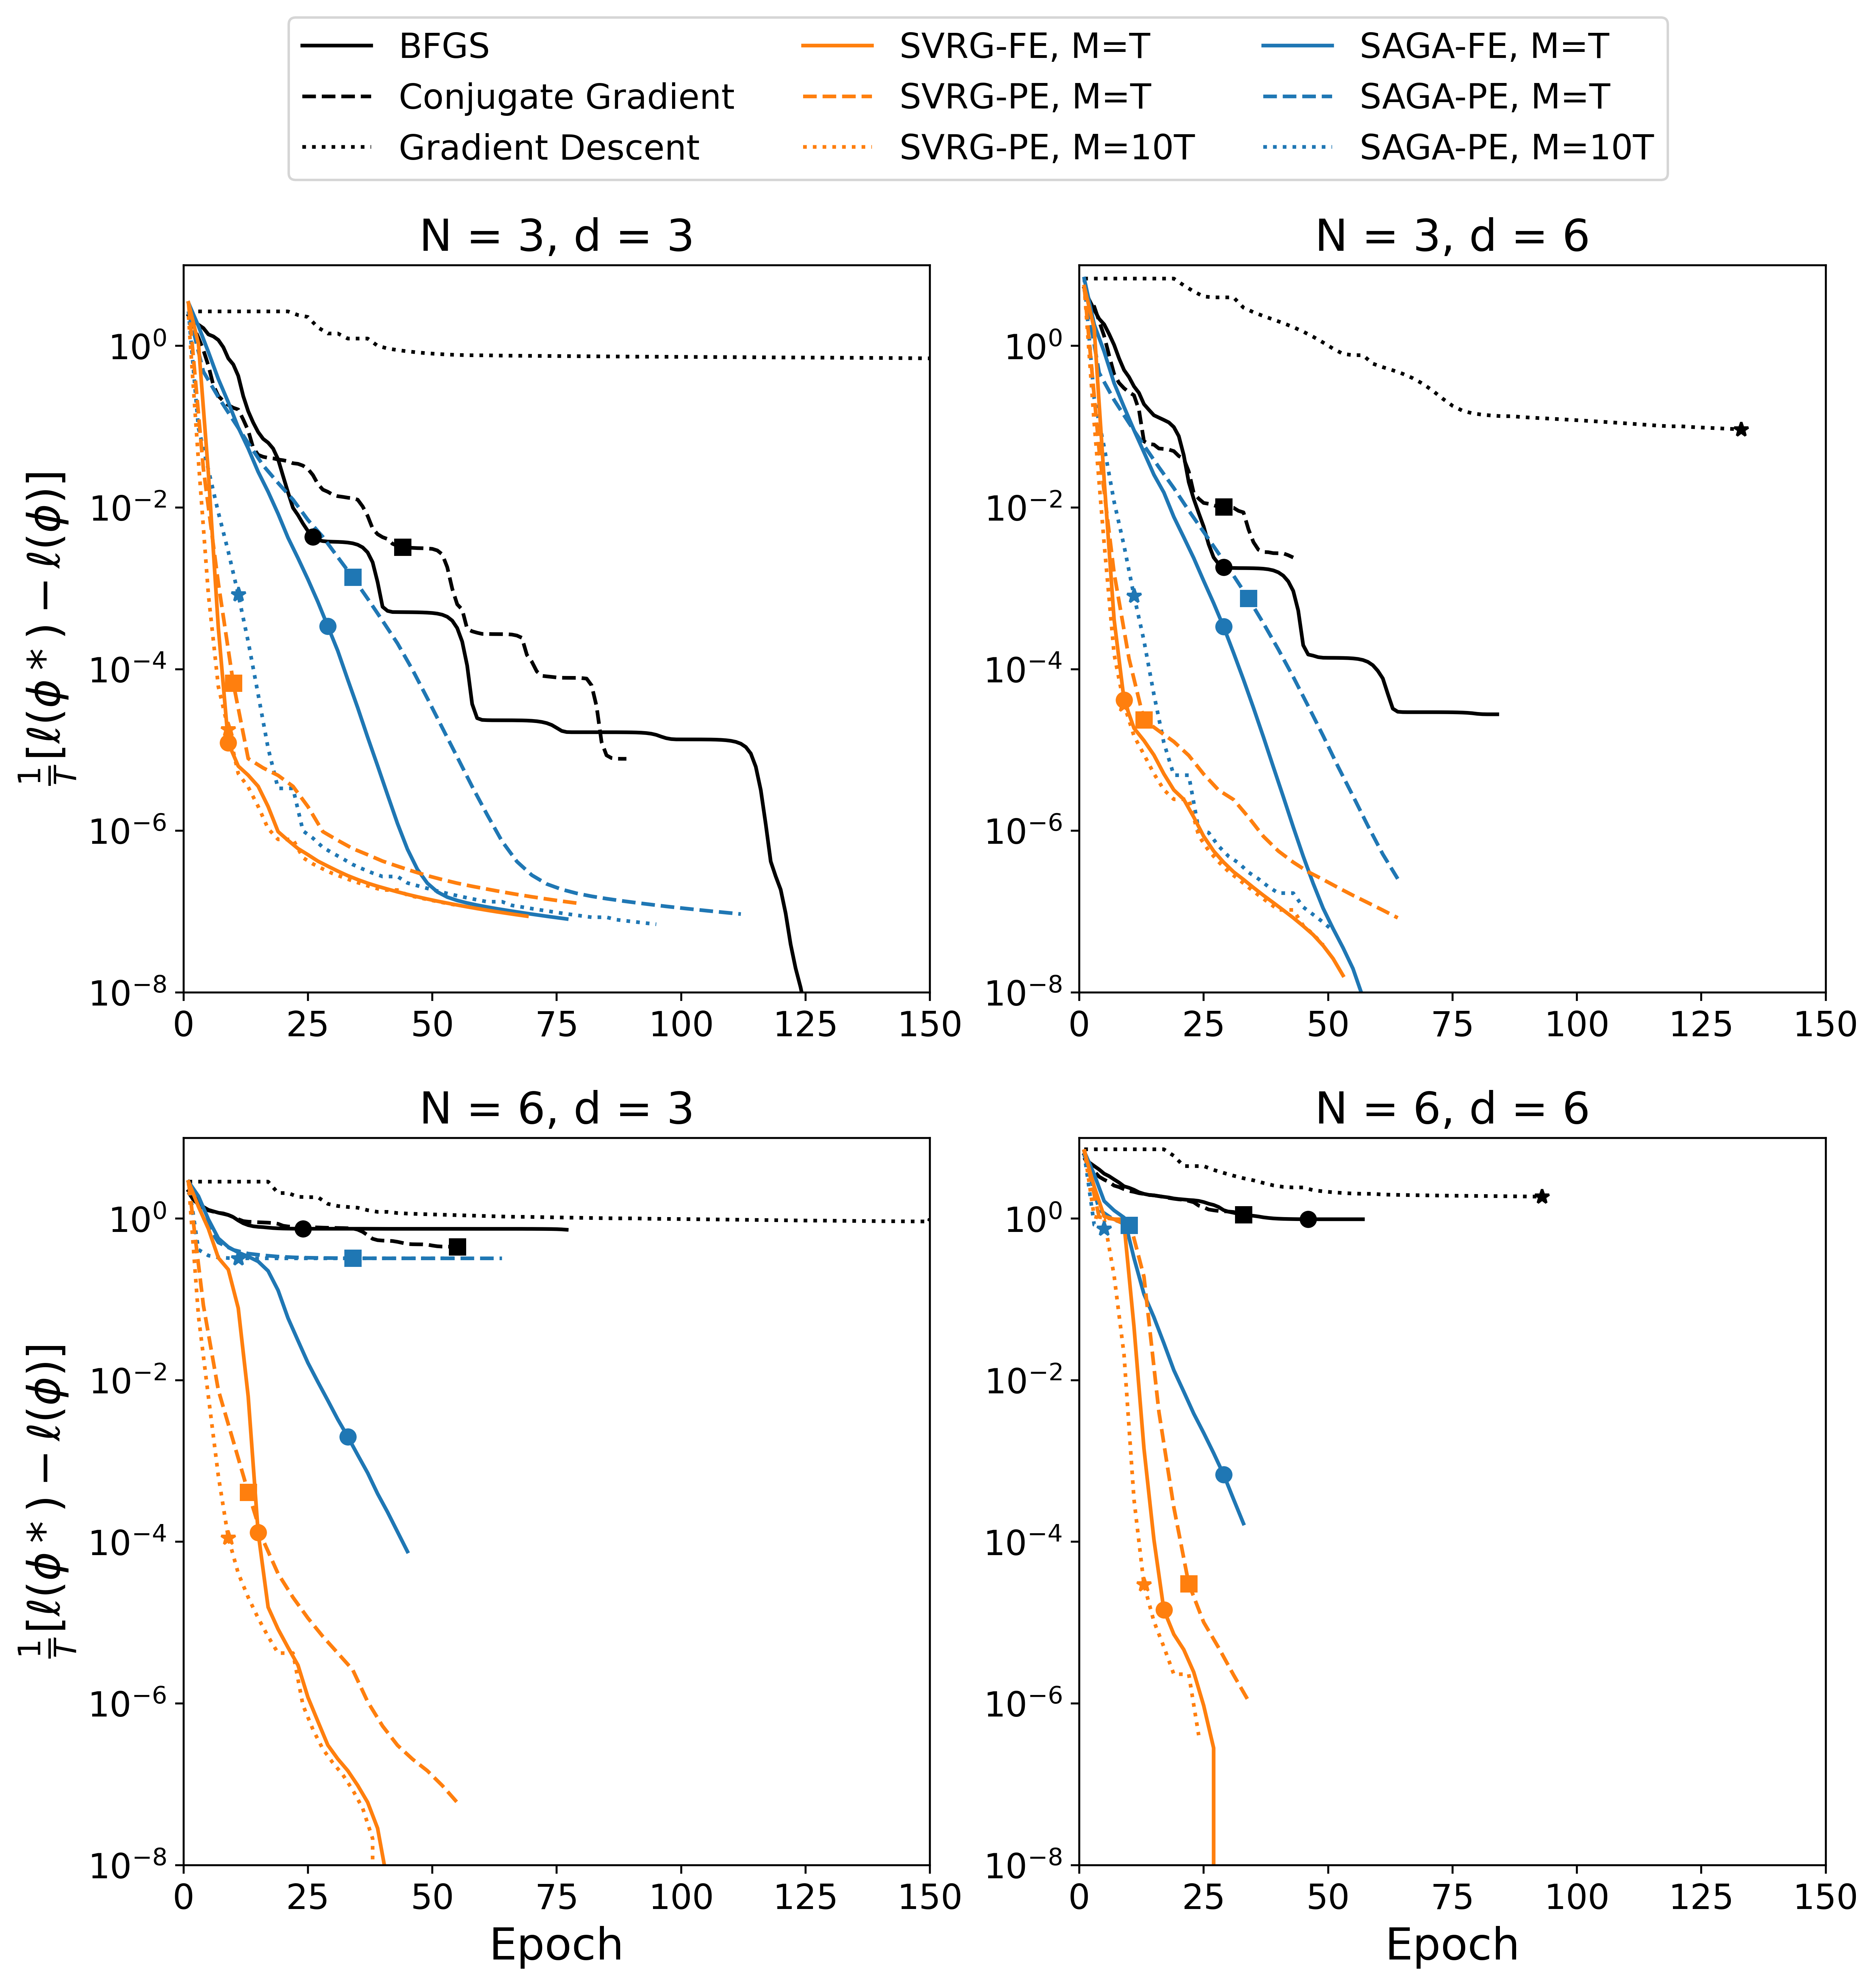
\includegraphics[width=5.5in]{../plt/log-like_v_epoch_T-100000-000.png}
    \caption{
    Maximum log-likelihood (across all algorithms and initial values after 12 hours), $\ell(\bfphi^*)$, minus the log-likelihood at the given epoch, $\ell(\bfphi)$, divided by $T$ for a selected run of each optimization algorithm in the simulation study. 
    Each algorithm was run for 12 hours on a data set generated with $T=10^{5}$, $N \in \{3,6\}$, or $d \in \{3,6\}$. For each experiment and optimization algorithm, we display the one random initialization (of five) that resulted in the highest likelihood after 12 hours}. FE corresponds to $P = \texttt{False}$, and PE corresponds to $P = \texttt{True}$. The y-axis is on a log-scale. Dots correspond to the epoch and likelihood at termination. 
    \label{fig:ll_trace_sim}
\end{figure}
%
\begin{figure}%[ht]
    \centering
    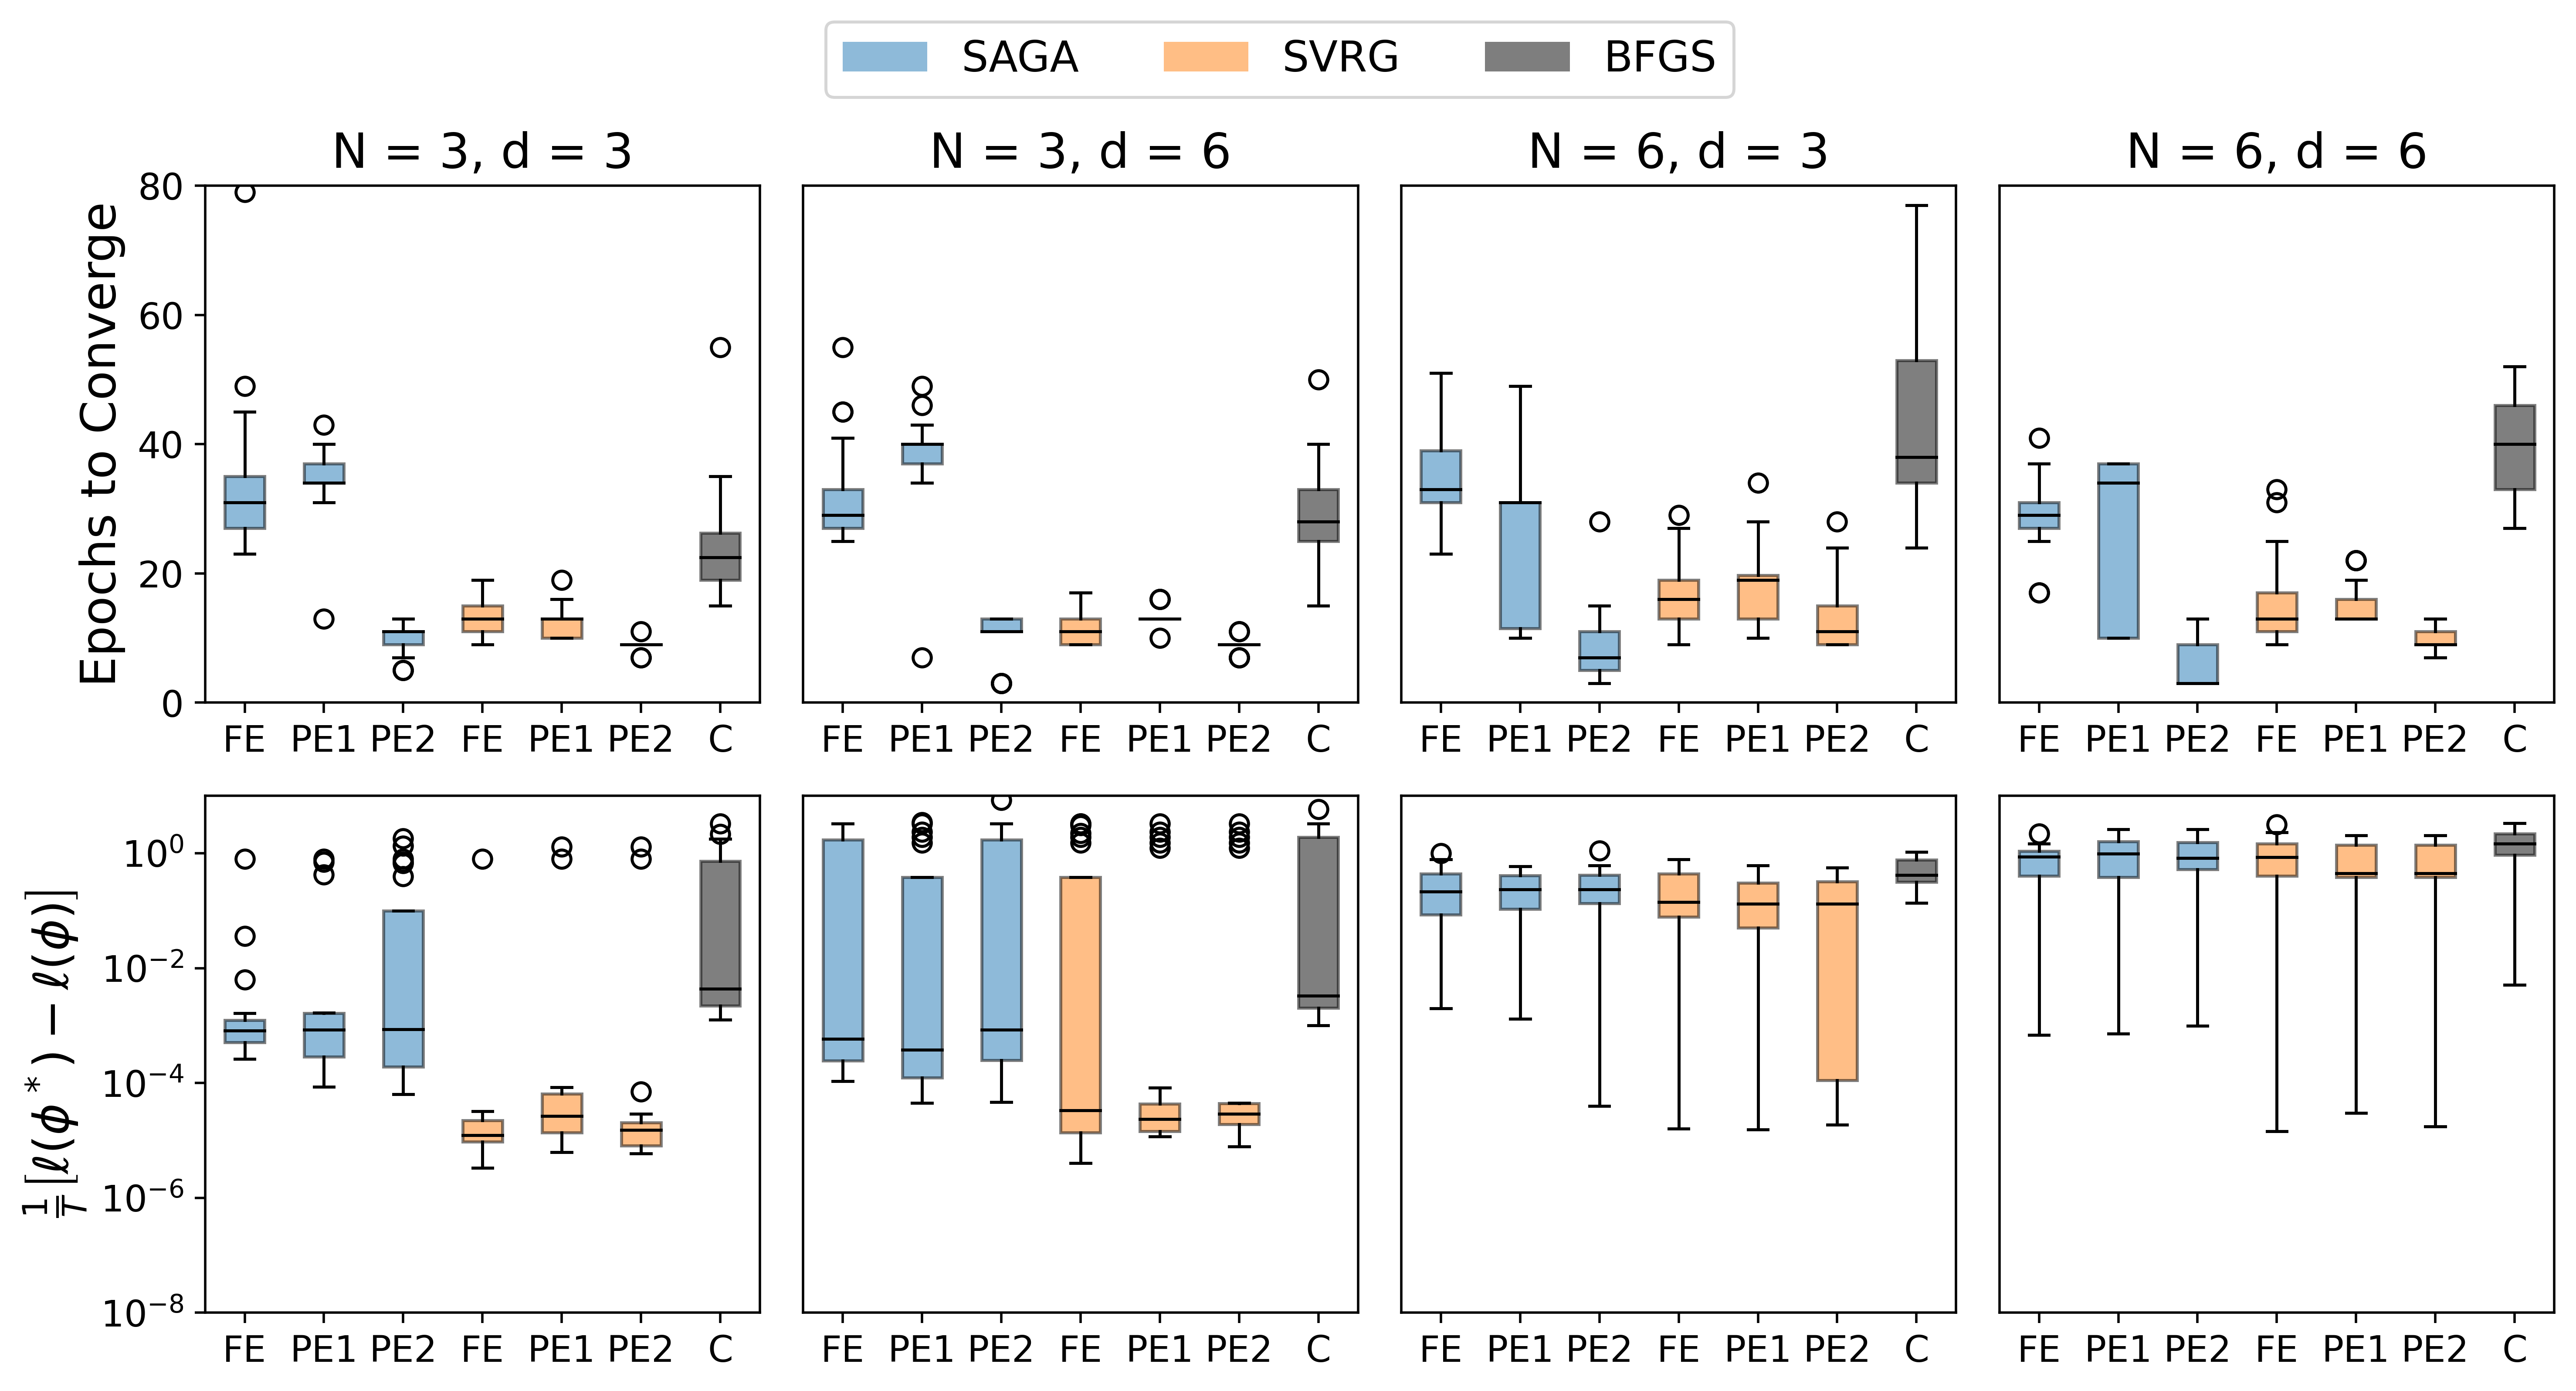
\includegraphics[width=6.5in]{../plt/boxplots_sim_T_100000.png}
    \caption{Box plots showing time to terminate (top), epochs to terminate (middle), and maximum log-likelihood minus log-likelihood at termination (all over $T$, bottom) for each optimization algorithm in the simulation study. The log-likelihood is denoted as $\ell(\bfphi)$, and the maximum log-likelihood across all algorithms and initial values after 12 hours is denoted as $\ell(\bfphi^*)$. Unlike Figure \ref{fig:ll_trace_sim}, results include all five data sets and all five parameter initializations per data set}. FE corresponds to $\{P = \texttt{False}, M = T\}$, PE1 corresponds to $\{P = \texttt{True}, M = T\}$, and PE2 corresponds to $\{P = \texttt{False}, M = 10T\}$. Results are shown for all simulation studies with $T=10^{5}$. The y-axis of the bottom row is on a log-scale.
    \label{fig:boxplots_sim}
\end{figure}
%
\begin{figure}%[ht]
    \centering
    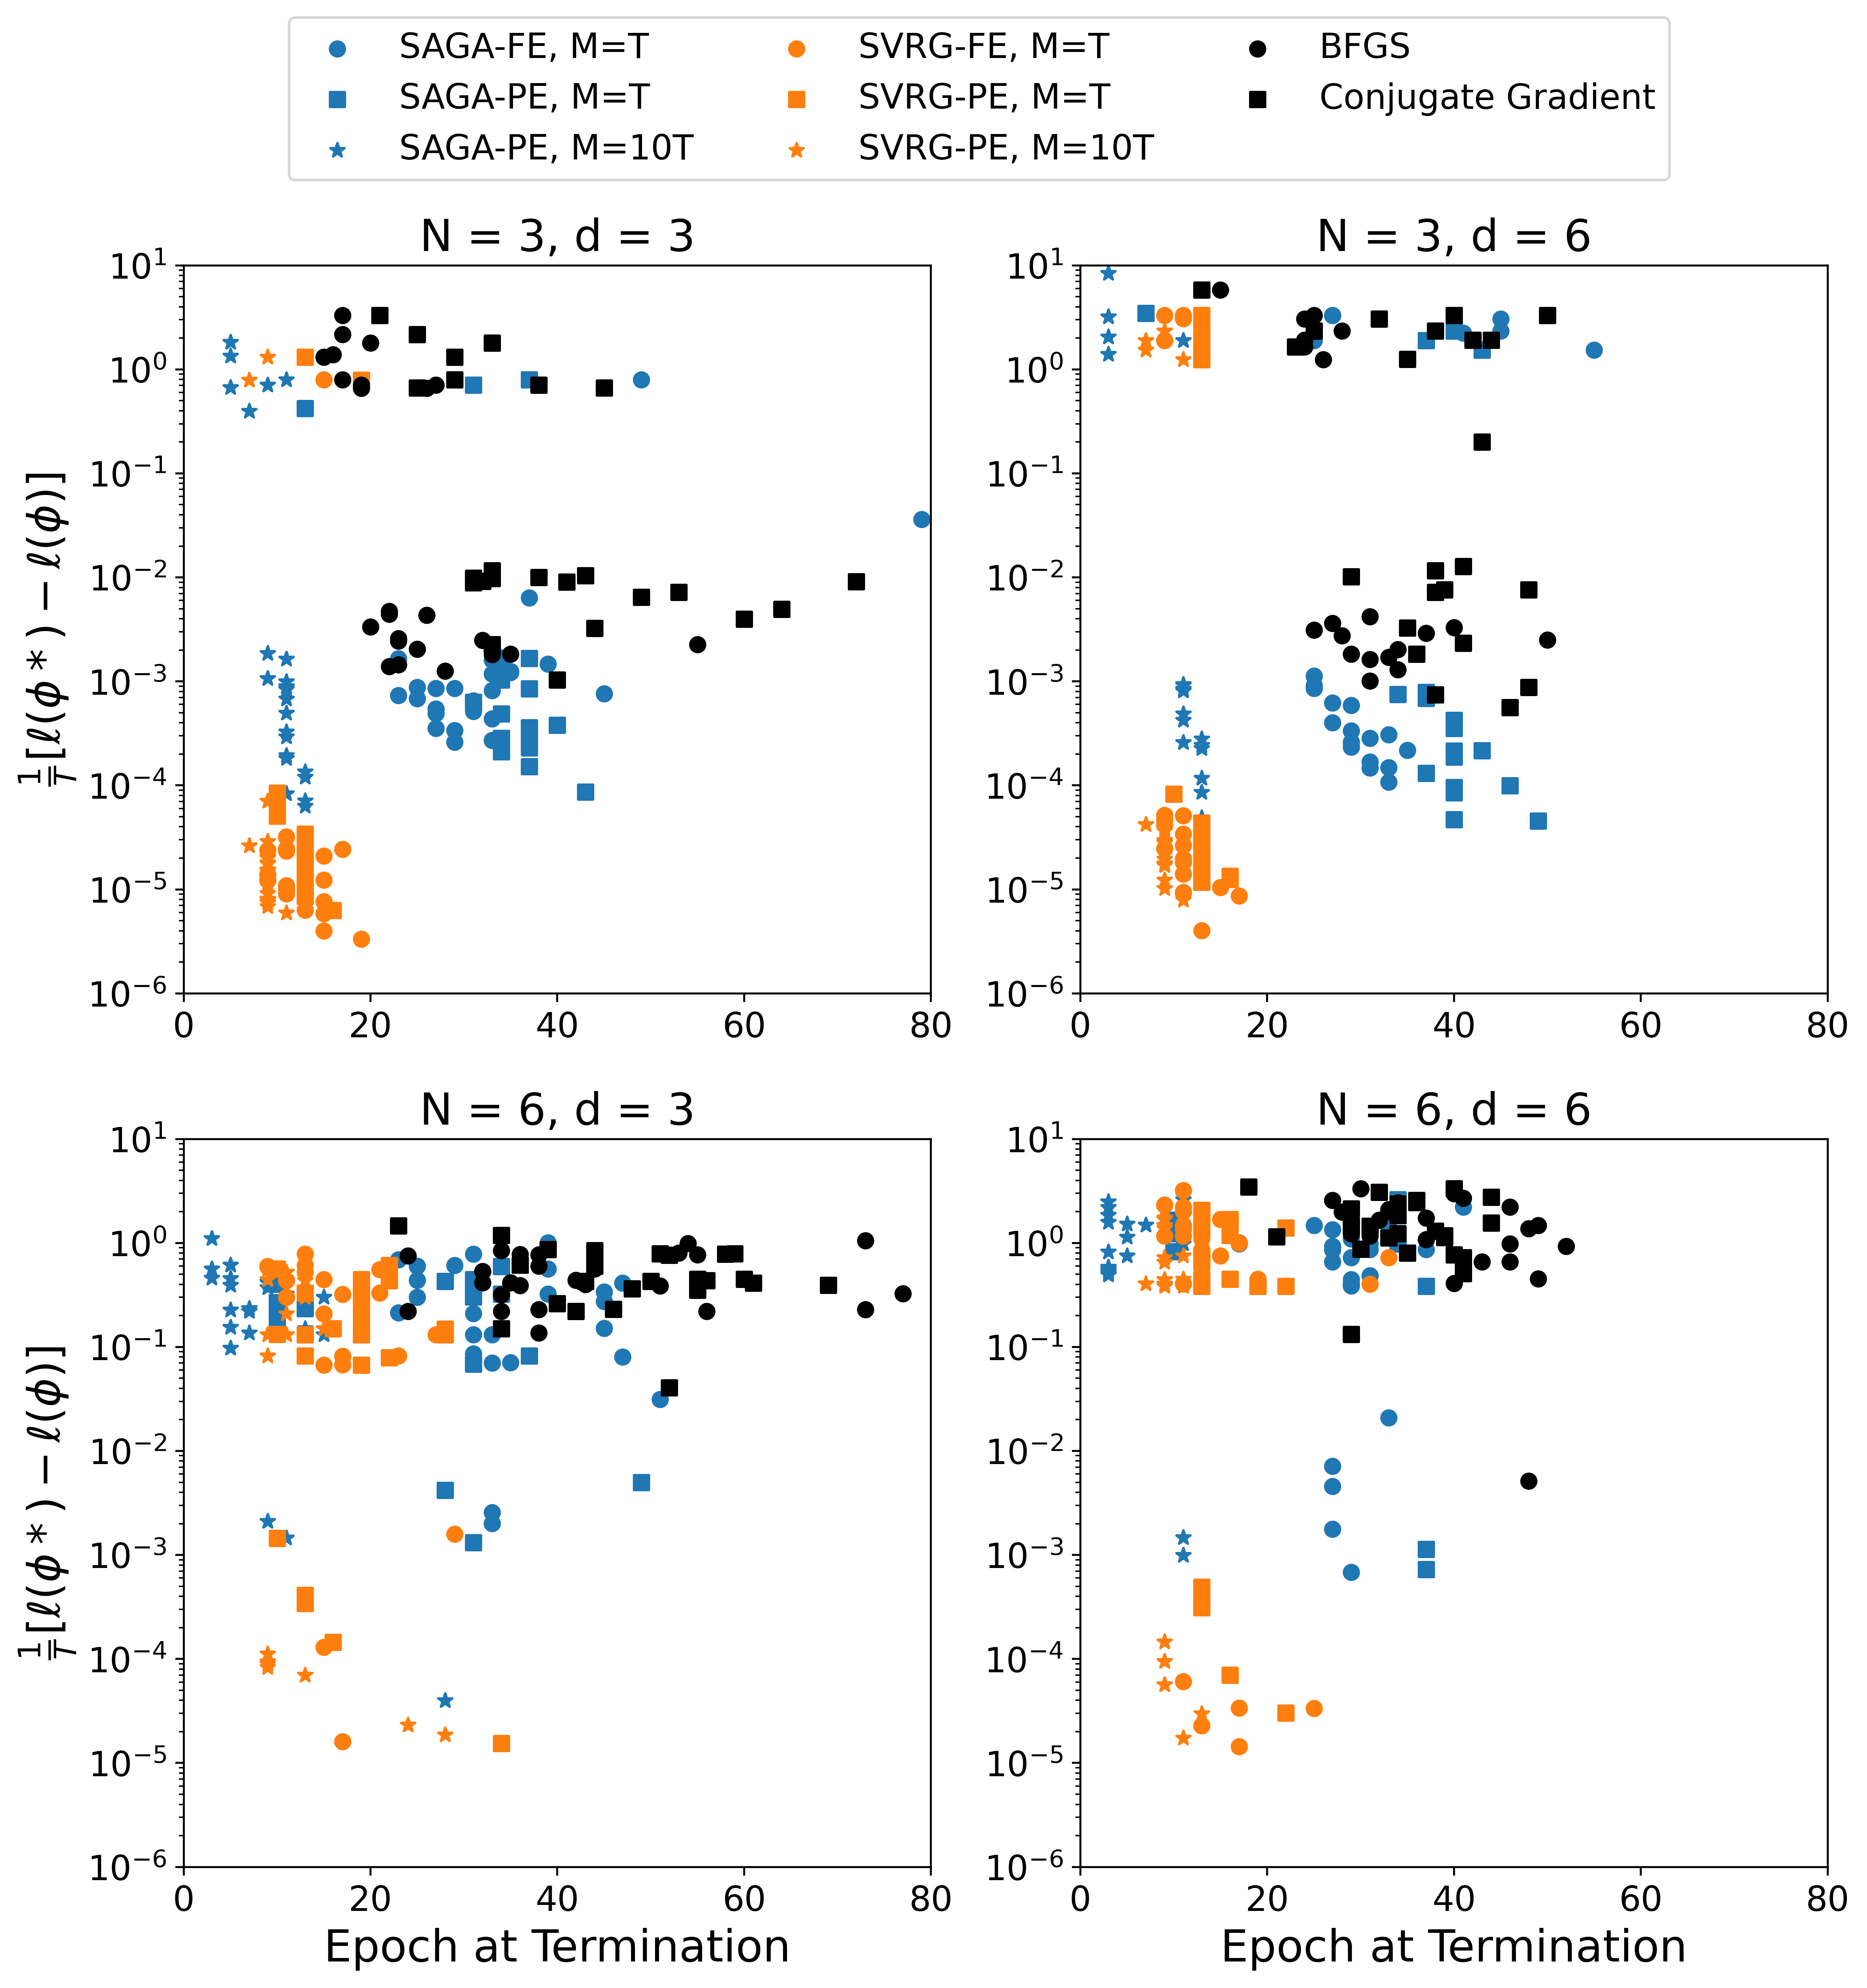
\includegraphics[width=5.5in]{../plt/scatter_sim_T_100000_epoch.png}
    \caption{Maximum log-likelihood minus log-likelihood at termination (all over $T$) versus epochs to terminate for each optimization algorithm in the simulation study with $T=10^{5}$, $N \in \{3,6\}$, and $d \in \{3,6\}$. The log-likelihood is denoted as $\ell(\bfphi)$, and the maximum log-likelihood across all algorithms and initial values after 12 hours is denoted as $\ell(\bfphi^*)$. Unlike Figure \ref{fig:ll_trace_sim}, results include all five data sets and all five parameter initializations per data set}. FE corresponds to $P = \texttt{False}$, and PE corresponds to $P = \texttt{True}$. The y-axis is on a log-scale.
    \label{fig:scatter_sim}
\end{figure}
%
Algorithm \ref{alg:EM-VRSO} with $A=\text{SVRG}$ markedly sped up the optimization procedure, as it usually converged in at most half as many epochs compared to the baselines for each experiment. Algorithm \ref{alg:EM-VRSO} with $A=\text{SAGA}$ also tended to converge in fewer epochs than the baselines for experiments with $N=6$, particularly when $P = \texttt{True}$ and $M=10T$. One epoch of each baseline method took less computation time than one epoch of Algorithm \ref{alg:EM-VRSO}, but Algorithm \ref{alg:EM-VRSO} with $A=\text{SVRG}$ consistently converged before the baseline methods in terms of raw computation time as well as epoch (Figure \ref{fig:boxplots_sim} and Supplement A).
%
All methods were prone to converge to local minima of the negative log likelihood, especially when $N=6$, in which case the likelihood surface was highly multi-modal. However, the bottom row of Figure \ref{fig:boxplots_sim} shows that in all $T=10^5$ experiments, negative log-likelihood values at termination were lower for all versions of Algorithm \ref{alg:EM-VRSO} compared to baseline methods. In particular, each optimization algorithm / experiment pair has a corresponding box plot which summarizes the (re-scaled) negative log-likelihood values at termination from all data sets and initializations. For all experiments, all medians and minimums corresponding to versions of Algorithm \ref{alg:EM-VRSO} were lower than the median and minimum values corresponding to BFGS. The results for experiments with $T=10^3$ were more varied (see Figure 1 of Supplement A), which indicates that our inference method is more efficient when applied to data sets with large $T$.
%
We present figures analogous to Figure \ref{fig:ll_trace_sim} for all five data sets corresponding to all experiments in Supplement A.